\subsection{Introducción}

  \paragraph{}El usuario \textit{Alumno} se encarga de gestionar su propia
  información y de responder a las entrevistas que le sean realizadas por su
  asesor, en un determinado curso académico. La información que puede gestionar
  este usuario se menciona a continuación:

  \begin{itemize}
   \item Matrículas
   \begin{itemize}
      \item Matriculación actual
      \item Matriculación histórica
   \end{itemize}
   \item Reuniones
  \end{itemize}

  \paragraph{}Además, a este usuario le estará permitido modificar completamente
  su información personal, con objeto de facilitar la labor de asesoría a su
  asesor.

  \paragraph{}Para acceder a cada uno de estos elementos, se podrá realizar de
  dos formas distintas:

  \begin{itemize}
   \item Mediante el menú principal. Este menú es el que refleja la figura
   \ref{capturaMenuPrincipalAlumno}.

  \begin{figure}[!ht]
    \begin{center}
      
\includegraphics[scale=0.55]{4.Funcionamiento_Aplicacion/4.3.Gestion/4.3.4.Alumno/4.3.4.1.Introduccion/menu_principal.png}
      \caption{Captura del menú principal del usuario \textit{Asesor}.}
      \label{capturaMenuPrincipalAlumno}
    \end{center}
  \end{figure}

   \item Mediante el menú lateral. Este menú es el que refleja la figura
   \ref{capturaMenuLateralAlumno}.

   \begin{figure}[!ht]
    \begin{center}
      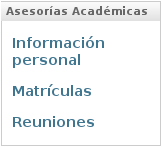
\includegraphics[scale=0.55]{4.Funcionamiento_Aplicacion/4.3.Gestion/4.3.4.Alumno/4.3.4.1.Introduccion/menu_lateral.png}
      \caption{Captura del menú lateral del usuario \textit{Alumno}.}
      \label{capturaMenuLateralAlumno}
    \end{center}
  \end{figure}

  \end{itemize}

  \paragraph{}A continuación, se pasa a detallar todos y cada uno de los
  elementos que este usuario puede gestionar en el sistema.
